\documentclass[12pt]{article}
\usepackage[paperwidth=13.333in,paperheight=7.5in,margin=0in]{geometry}
\usepackage[T1]{fontenc}
\usepackage{lmodern}
\usepackage{amsmath,amssymb}
\usepackage{graphicx}
\usepackage{xcolor}
\usepackage{tikz}
\usepackage{helvet}
\renewcommand{\familydefault}{\sfdefault}
\pagestyle{empty}
\setlength{\parindent}{0pt}
\usetikzlibrary{positioning,calc,fit,backgrounds}
\definecolor{markovadd}{HTML}{4C78A8}
\definecolor{markovneural}{HTML}{E45756}
\definecolor{ctreegreen}{HTML}{54A24B}
\definecolor{guideorange}{HTML}{F58518}
\definecolor{softgray}{HTML}{F4F6F8}
\definecolor{midgray}{HTML}{D9DEE3}
\newcommand{\slidebox}[4]{
  \node[anchor=north west, rounded corners=7pt, draw=#1!70!black, fill=#1!8, line width=0.9pt, inner sep=10pt,
        align=left] at #3 {\parbox{#2}{\raggedright #4}};
}
\begin{document}
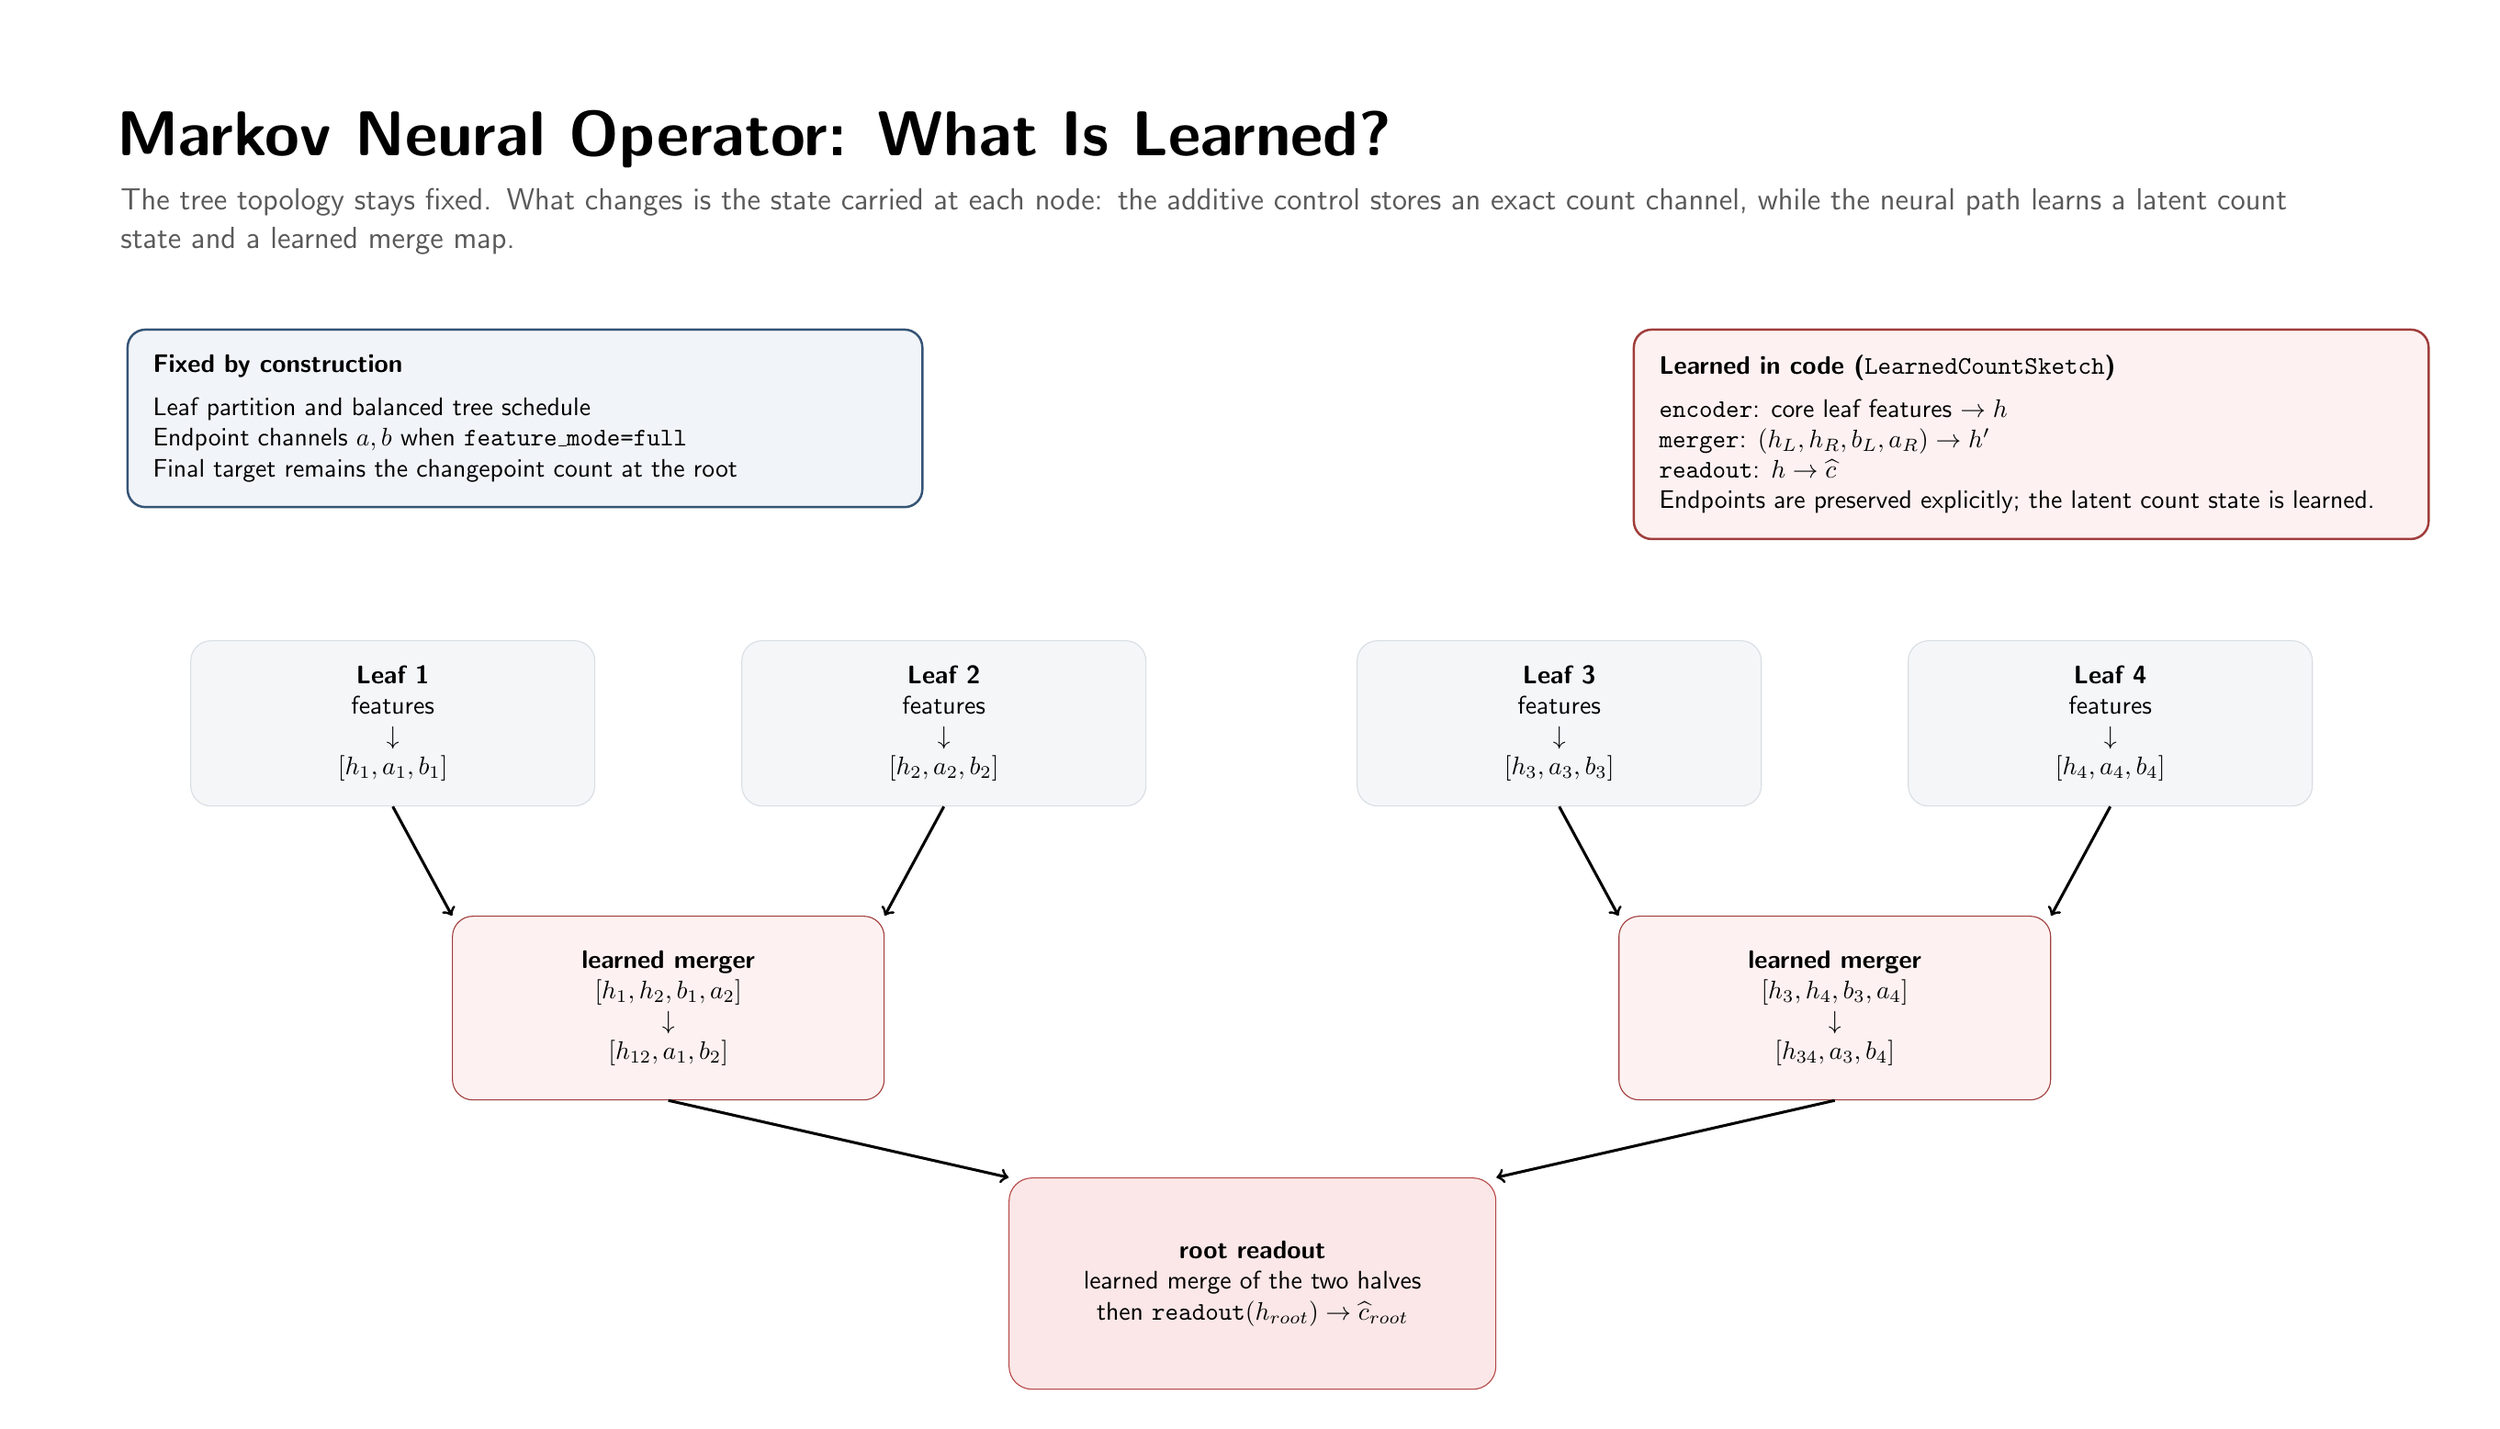
\begin{tikzpicture}[x=1in,y=1in]
\useasboundingbox (0,0) rectangle (13.333,7.5);

\node[anchor=north west, font=\bfseries\fontsize{26}{28}\selectfont] at (0.45,7.08) {Markov Neural Operator: What Is Learned?};
\node[anchor=north west, text=black!65, font=\fontsize{13}{15}\selectfont, text width=12.15in] at (0.47,6.66) {The tree topology stays fixed. What changes is the state carried at each node: the additive control stores an exact count channel, while the neural path learns a latent count state and a learned merge map.};
\slidebox{markovadd}{4.05in}{(0.55,5.85)}{\bfseries Fixed by construction\\[0.45em]\mdseries Leaf partition and balanced tree schedule\\ Endpoint channels $a,b$ when \texttt{feature\_mode=full}\\ Final target remains the changepoint count at the root}
\slidebox{markovneural}{4.05in}{(8.75,5.85)}{\bfseries Learned in code (\texttt{LearnedCountSketch})\\[0.45em]\mdseries \texttt{encoder}: core leaf features $\rightarrow h$\\ \texttt{merger}: $(h_L,h_R,b_L,a_R)\rightarrow h'$\\ \texttt{readout}: $h \rightarrow \widehat{c}$\\ Endpoints are preserved explicitly; the latent count state is learned.}
\node[draw=midgray, fill=softgray, rounded corners=8pt, minimum width=2.2in, minimum height=0.9in, align=center] (leaf1) at (2.0,3.7) {{\bfseries Leaf 1}\\ features\\ $\downarrow$\\ $[h_1,a_1,b_1]$};
\node[draw=midgray, fill=softgray, rounded corners=8pt, minimum width=2.2in, minimum height=0.9in, align=center] (leaf2) at (5.0,3.7) {{\bfseries Leaf 2}\\ features\\ $\downarrow$\\ $[h_2,a_2,b_2]$};
\node[draw=markovneural!70!black, fill=markovneural!8, rounded corners=8pt, minimum width=2.35in, minimum height=1.0in, align=center] (merge12) at (3.5,2.15) {{\bfseries learned merger}\\ $[h_1,h_2,b_1,a_2]$\\ $\downarrow$\\ $[h_{12},a_1,b_2]$};
\node[draw=midgray, fill=softgray, rounded corners=8pt, minimum width=2.2in, minimum height=0.9in, align=center] (leaf3) at (8.35,3.7) {{\bfseries Leaf 3}\\ features\\ $\downarrow$\\ $[h_3,a_3,b_3]$};
\node[draw=midgray, fill=softgray, rounded corners=8pt, minimum width=2.2in, minimum height=0.9in, align=center] (leaf4) at (11.35,3.7) {{\bfseries Leaf 4}\\ features\\ $\downarrow$\\ $[h_4,a_4,b_4]$};
\node[draw=markovneural!70!black, fill=markovneural!8, rounded corners=8pt, minimum width=2.35in, minimum height=1.0in, align=center] (merge34) at (9.85,2.15) {{\bfseries learned merger}\\ $[h_3,h_4,b_3,a_4]$\\ $\downarrow$\\ $[h_{34},a_3,b_4]$};
\node[draw=markovneural!80!black, fill=markovneural!14, rounded corners=9pt, minimum width=2.65in, minimum height=1.15in, align=center] (root) at (6.68,0.65) {{\bfseries root readout}\\ learned merge of the two halves\\ then \texttt{readout}$(h_{root})\rightarrow \widehat{c}_{root}$};
\draw[->, line width=1.1pt] (leaf1.south) -- (merge12.north west);
\draw[->, line width=1.1pt] (leaf2.south) -- (merge12.north east);
\draw[->, line width=1.1pt] (leaf3.south) -- (merge34.north west);
\draw[->, line width=1.1pt] (leaf4.south) -- (merge34.north east);
\draw[->, line width=1.1pt] (merge12.south) -- (root.north west);
\draw[->, line width=1.1pt] (merge34.south) -- (root.north east);
\end{tikzpicture}
\end{document}
